% !TeX document-id = {c68f4be8-c497-43e0-82df-e9ebfbea9577}
% !TeX TXS-program:pdflatex = pdflatex -synctex=1 -interaction=nonstopmode --shell-escape %.tex
% новая команда \RNumb для вывода римских цифр
\documentclass[a4paper,12pt]{article}
\usepackage{amssymb}
\usepackage{amsmath}
\usepackage{amsthm}
\usepackage{caption}
\usepackage{misccorr}
\usepackage[noadjust]{cite}
\usepackage{cmap}
\usepackage[utf8x]{inputenc}
\usepackage[T2A]{fontenc}
\usepackage[english, russian]{babel}
\usepackage{graphics}
\usepackage{graphicx}
\usepackage{textcomp}
\usepackage{verbatim}
\usepackage{makeidx}
\usepackage{geometry}
\usepackage{float}
\usepackage{bm}
\usepackage{esint}
\usepackage{mathtools}
\usepackage{graphicx}
\usepackage{listings}
\usepackage{courier}
\usepackage{multirow}
\usepackage{graphicx}
\usepackage{xcolor}
\usepackage{ucs}


\lstdefinestyle{asm}{
	language={[x86masm]Assembler},
	backgroundcolor=\color{white},
	basicstyle=\footnotesize\ttfamily,
	keywordstyle=\color{blue},
	stringstyle=\color{red},
	commentstyle=\color{gray},
	numbers=left,
	numberstyle=\tiny,
	stepnumber=1,
	numbersep=5pt,
	frame=single,
	tabsize=4,
	captionpos=b,
	breaklines=true
}

\lstset{basicstyle=\fontsize{10}{10}\selectfont,breaklines=true,inputencoding=utf8x,extendedchars=\true}

\lstset{
	literate=
	{а}{{\selectfont\char224}}1
	{б}{{\selectfont\char225}}1
	{в}{{\selectfont\char226}}1
	{г}{{\selectfont\char227}}1
	{д}{{\selectfont\char228}}1
	{е}{{\selectfont\char229}}1
	{ё}{{\"e}}1
	{ж}{{\selectfont\char230}}1
	{з}{{\selectfont\char231}}1
	{и}{{\selectfont\char232}}1
	{й}{{\selectfont\char233}}1
	{к}{{\selectfont\char234}}1
	{л}{{\selectfont\char235}}1
	{м}{{\selectfont\char236}}1
	{н}{{\selectfont\char237}}1
	{о}{{\selectfont\char238}}1
	{п}{{\selectfont\char239}}1
	{р}{{\selectfont\char240}}1
	{с}{{\selectfont\char241}}1
	{т}{{\selectfont\char242}}1
	{у}{{\selectfont\char243}}1
	{ф}{{\selectfont\char244}}1
	{х}{{\selectfont\char245}}1
	{ц}{{\selectfont\char246}}1
	{ч}{{\selectfont\char247}}1
	{ш}{{\selectfont\char248}}1
	{щ}{{\selectfont\char249}}1
	{ъ}{{\selectfont\char250}}1
	{ы}{{\selectfont\char251}}1
	{ь}{{\selectfont\char252}}1
	{э}{{\selectfont\char253}}1
	{ю}{{\selectfont\char254}}1
	{я}{{\selectfont\char255}}1
	{А}{{\selectfont\char192}}1
	{Б}{{\selectfont\char193}}1
	{В}{{\selectfont\char194}}1
	{Г}{{\selectfont\char195}}1
	{Д}{{\selectfont\char196}}1
	{Е}{{\selectfont\char197}}1
	{Ё}{{\"E}}1
	{Ж}{{\selectfont\char198}}1
	{З}{{\selectfont\char199}}1
	{И}{{\selectfont\char200}}1
	{Й}{{\selectfont\char201}}1
	{К}{{\selectfont\char202}}1
	{Л}{{\selectfont\char203}}1
	{М}{{\selectfont\char204}}1
	{Н}{{\selectfont\char205}}1
	{О}{{\selectfont\char206}}1
	{П}{{\selectfont\char207}}1
	{Р}{{\selectfont\char208}}1
	{С}{{\selectfont\char209}}1
	{Т}{{\selectfont\char210}}1
	{У}{{\selectfont\char211}}1
	{Ф}{{\selectfont\char212}}1
	{Х}{{\selectfont\char213}}1
	{Ц}{{\selectfont\char214}}1
	{Ч}{{\selectfont\char215}}1
	{Ш}{{\selectfont\char216}}1
	{Щ}{{\selectfont\char217}}1
	{Ъ}{{\selectfont\char218}}1
	{Ы}{{\selectfont\char219}}1
	{Ь}{{\selectfont\char220}}1
	{Э}{{\selectfont\char221}}1
	{Ю}{{\selectfont\char222}}1
	{Я}{{\selectfont\char223}}1
}

\newcommand{\specchapter}[1]{\chapter*{#1}\addcontentsline{toc}{chapter}{#1}}
\newcommand{\specsection}[1]{\section*{#1}\addcontentsline{toc}{section}{#1}}
\newcommand{\specsubsection}[1]{\subsection*{#1}\addcontentsline{toc}{subsection}{#1}}
\newcommand{\RNumb}[1]{\uppercase\expandafter{\romannumeral #1\relax}}
\newcommand{\jj}{\righthyphenmin=20 \justifying}


% геометрия
\geometry{pdftex, left = 2cm, right = 2cm, top = 2.5cm, bottom = 2.5cm}

\setcounter{tocdepth}{4} % фикс переноса 
\righthyphenmin = 2
\tolerance = 2048

\begin{document}
\thispagestyle{empty}

\noindent \begin{minipage}{0.15\textwidth}
	
\includegraphics[width=\linewidth]{b_logo}
\end{minipage}
\noindent\begin{minipage}{0.9\textwidth}\centering
	\textbf{Министерство науки и высшего образования Российской Федерации}\\
	\textbf{Федеральное государственное бюджетное образовательное учреждение высшего образования}\\
	\textbf{«Московский государственный технический университет имени Н.Э.~Баумана}\\
	\textbf{(национальный исследовательский университет)»}\\
	\textbf{(МГТУ им. Н.Э.~Баумана)}
\end{minipage}

\noindent\rule{18cm}{3pt}
\newline\newline
\noindent ФАКУЛЬТЕТ $\underline{\text{«Информатика и системы управления»}}$ \newline\newline
\noindent КАФЕДРА $\underline{\text{«Программное обеспечение ЭВМ и информационные технологии»}}$\newline\newline\newline\newline\newline\newline\newline


\begin{center}
	\noindent\begin{minipage}{1.3\textwidth}\centering
	\Large\textbf{   ~~~ Лабораторная работа №1}\newline
	\textbf{по дисциплине "Операционные системы"}\newline\newline\newline
	\end{minipage}
\end{center}

\noindent\textbf{Тема} $\underline{\text{Дизассемблирование INT 8h}}$\newline\newline
\noindent\textbf{Студент} $\underline{\text{Рядинский К. В.}}$\newline\newline
\noindent\textbf{Группа} $\underline{\text{ИУ7-53Б}}$\newline\newline
\noindent\textbf{Преподаватель} $\underline{\text{Рязанова Н.Ю.}}$\newline

\begin{center}
	\vfill
	Москва~---~\the\year
~г.
\end{center}
\clearpage

\section{Полученный дизассемблированный код}

\subsection{Листинг INT8h} 
\begin{lstlisting}[style={asm}]
	020A:0746	;*		call	sub_1			; (07B9)
020A:0746			db	0E8h, 70h, 00h

; сохранение регистров
020A:0749			push	es
020A:074A			push	ds
020A:074B			push	ax
020A:074C			push	dx
020A:074D			mov	ax,40h
020A:0750			mov	ds,ax
020A:0752			xor	ax,ax			; Zero register
020A:0754			mov	es,ax

; инкремент счетчика таймера реального времени
020A:0756			inc	word ptr ds:[6Ch]	
; (0040:006C=2E56h), по этому адресу располагается счетчик реального времени
020A:075A			jnz	loc_1			; Jump if not zero
;если значение  в 0040:006C равно нулю, то инкрементируются старшие 2 байта
020A:075C			inc	word ptr ds:[6Eh]	; (0040:006E=2)

; сброс счетчика таймера реального времени, если наступили новые сутки
020A:0760	loc_1:
020A:0760			cmp	word ptr ds:[6Eh],18h	; (0040:006E=2)
020A:0765			jne	loc_2			; Jump if not equal
020A:0767			cmp	word ptr ds:[6Ch],0B0h	; (0040:006C=2E56h)
020A:076D			jne	loc_2			; Jump if not equal
; прошло более 24 часов с момента запуска таймера, обнуление счетчика
020A:076F			mov	word ptr ds:[6Eh],ax	; (0040:006E=2)
020A:0772			mov	word ptr ds:[6Ch],ax	; (0040:006C=2E56h)
020A:0775			mov	byte ptr ds:[70h],1	; (0040:0070=0)
; в 0040:0070 хранится переполнения таймера (переход через 24 часа)
020A:077A			or	al,8



; декремент значения времени до выключения моторчика дисковода
020A:077C	loc_2:
020A:077C			push	ax
020A:077D			dec	byte ptr ds:[40h]	; (0040:0040=5Bh)
; ячейка с адресом 0040:0040 содержит время, оставшееся до выключения двигателя
020A:0781			jnz	loc_3			; Jump if not zero
; посыл команды на отключение моторчика дисковода
020A:0783			and	byte ptr ds:[3Fh],0F0h	; (0040:003F=0)
; в 0040:003F хранится состояние моторчика дисковода
020A:0788			mov	al,0Ch
020A:078A			mov	dx,3F2h
020A:078D			out	dx,al			; port 3F2h, dsk0 contrl output

; проверка на возможность вызова маскируемых прерываний
020A:078E	loc_3:
020A:078E			pop	ax
020A:078F			test	word ptr ds:[314h],4	; (0040:0314=3200h)
; ячейка с адресом 0040:0314 содержит информацию о значениях флагов (Проверка parity flag)
020A:0795			jnz	loc_4			; Jump if not zero
020A:0797			lahf				; Load ah from flags
; загрузка младшего байта регистра флагов в AH
; обмен ah и al
020A:0798			xchg	ah,al
020A:079A			push	ax
; косвенный вызов пользовательского прерывания
; Вызов 1Ch с помощью адреса в таблице векторов прерывания 
; При вызове через int произойдет сохранения регистра флагов в стек,
; а в случае вызова через call на его месте будет лежать сохраненный до ax
; который по выходе из 1Ch будет установлен в флаги через iret
020A:079B			call	dword ptr es:[70h]	; (0000:0070=6ADh)
020A:07A0			jmp	short loc_5		; (07A5)
020A:07A2			nop

; вызов пользовательского прерывания
020A:07A3	loc_4:
020A:07A3			int	1Ch			; Timer break (call each 18.2ms)

; сброс контроллера прерываний
020A:07A5	loc_5:
020A:07A5			call	sub_1			; (07B9)
020A:07A8			mov	al,20h			; ' '
020A:07AA			out	20h,al			; port 20h, 8259-1 int command
								;  al = 20h, end of interrupt
; восстановление регистров
020A:07AC			pop	dx
020A:07AD			pop	ax
020A:07AE			pop	ds
020A:07AF			pop	es
; переход по метке для завершения работы прерывания
020A:07B0			jmp	$-164h
020A:07B3			db	0C4h
					                        ;* No entry point to code
020A:07B4			les	cx,dword ptr ds:[93E9h]	; (0000:93E9=5A14h) Load 32 bit ptr
020A:07B8			db	0FEh

\end{lstlisting}

\clearpage
\subsection{Листинг процедуры sub\_1}

\begin{lstlisting}[style={asm}]
	sub_1		proc	near
	; сохранение регистров и загрузка регистра флагов
	020A:07B9			push	ds
	020A:07BA			push	ax
	020A:07BB			mov	ax,40h
	020A:07BE			mov	ds,ax
	020A:07C0			lahf				; Load ah from flags
	
	; проверка на возможность вызова маскируемых прерываний
	020A:07C1			test	word ptr ds:[314h],2400h; (0040:0314=3200h)
	020A:07C7			jnz	loc_7			; Jump if not zero
	; Сброс IEF (9 бит) lock для того, чтобы команда была неделимой
	020A:07C9	                    lock and word ptr ds:[314h],0FDFFh; (0040:0314=3200h)
	; установка флага IF в ноль
	
	; сохранение флагов и восстановление регистров
	020A:07D0	loc_6:
	020A:07D0			sahf				; Store ah into flags
	020A:07D1			pop	ax
	020A:07D2			pop	ds
	020A:07D3			jmp	short loc_8		; (07D8)
	
	
	; запрет на вызов маскируемых прерываний
	020A:07D5	loc_7:
	020A:07D5			cli				; Disable interrupts
	; сбрасывает interrupt flag (IF). Когда этот флаг сброшен процессор игнорирует все  
	; прерывания (кроме NMI) от внешних устройств.
	020A:07D6			jmp	short loc_6		; (07D0)
	
	; завершение процедуры
	020A:07D8	loc_8:
	020A:07D8			retn
			sub_1		endp
	
\end{lstlisting}
\clearpage

\section{Схема алгоритмов}

\subsection{Схема алгоритма обработчика INT8h}
""\newline

\begin{flushright}
	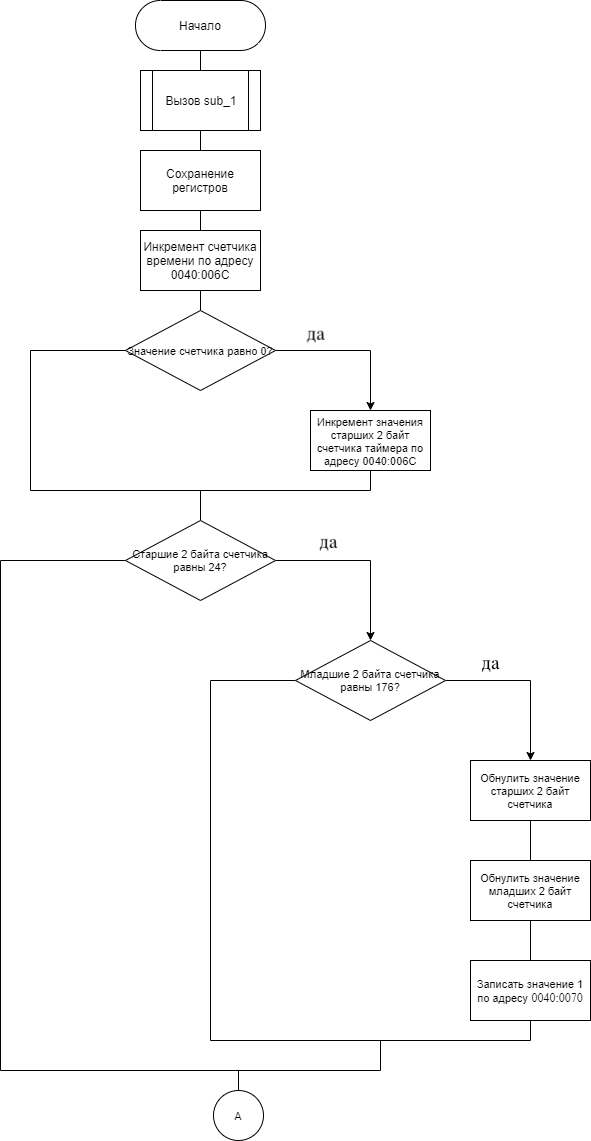
\includegraphics[scale=0.5]{scheme1.png}
	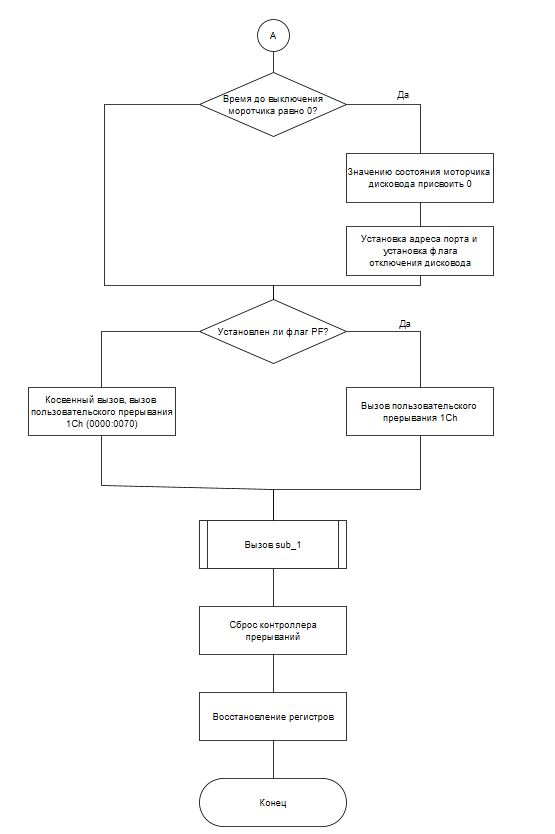
\includegraphics[scale=1]{scheme2.JPG}
\end{flushright}

\clearpage
\subsection{Схема алгоритма процедуры sub\_1}

\begin{center}
	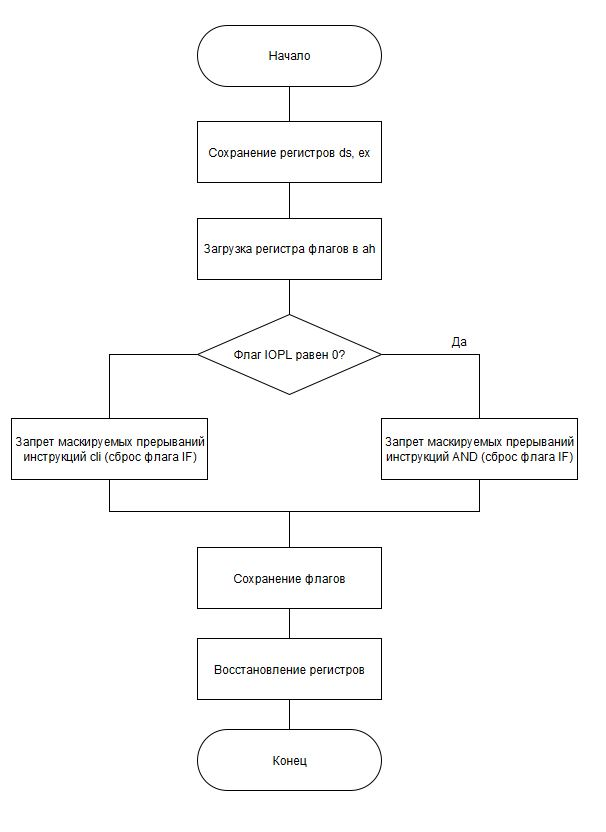
\includegraphics[scale=1]{scheme3.JPG}
\end{center}

\end{document}
